\section{Operación del transistor}

\subsection{BJT}
El transistor BJT se construye con tres regiones semiconductoras, separadas por
uniones \emph{pn}, las tres regiones se denominan \textbf{emisor}, \textbf{base}
y \textbf{colector}. Un tipo se compone de dos regiones \emph{n} separadas por
una región \emph{p} (\emph{npn}) y el otro tipo consta de dos regiones \emph{p}
separadas por una región \emph{n} (\emph{pnp}) como se muestra en la
\textbf{figura~\ref{figura01}} junto a sus símbolos esquemáticos \cite{Floyd}.

\begin{figure}[!ht]
\centering
\includegraphics[scale=0.30]{diagramas/figura01.eps}
\caption{Tipos de transistores BJT y sus símbolos estándar.}
\label{figura01}
\end{figure}

Cuando se conecta un transistor BJT a voltajes de polarización de cd, como se
muestra en la \textbf{figura~\ref{figura02}}, $V_{\text{BB}}$ polariza en
directa la unión base-emisor y $V_{\text{CC}}$ polariza en inversa la unión
base-colector.

Una reducción de la polarización en directo base-emisor provoca que la corriente
a través del transistor se reduzca en forma considerable. Por otra parte, al
incrementar la polarización en directo de la unión base-emisor reduce la barrera
de potencial y se permite el flujo de corriente a través del transistor
\cite{Savant}.

\begin{figure}[!ht]
\centering
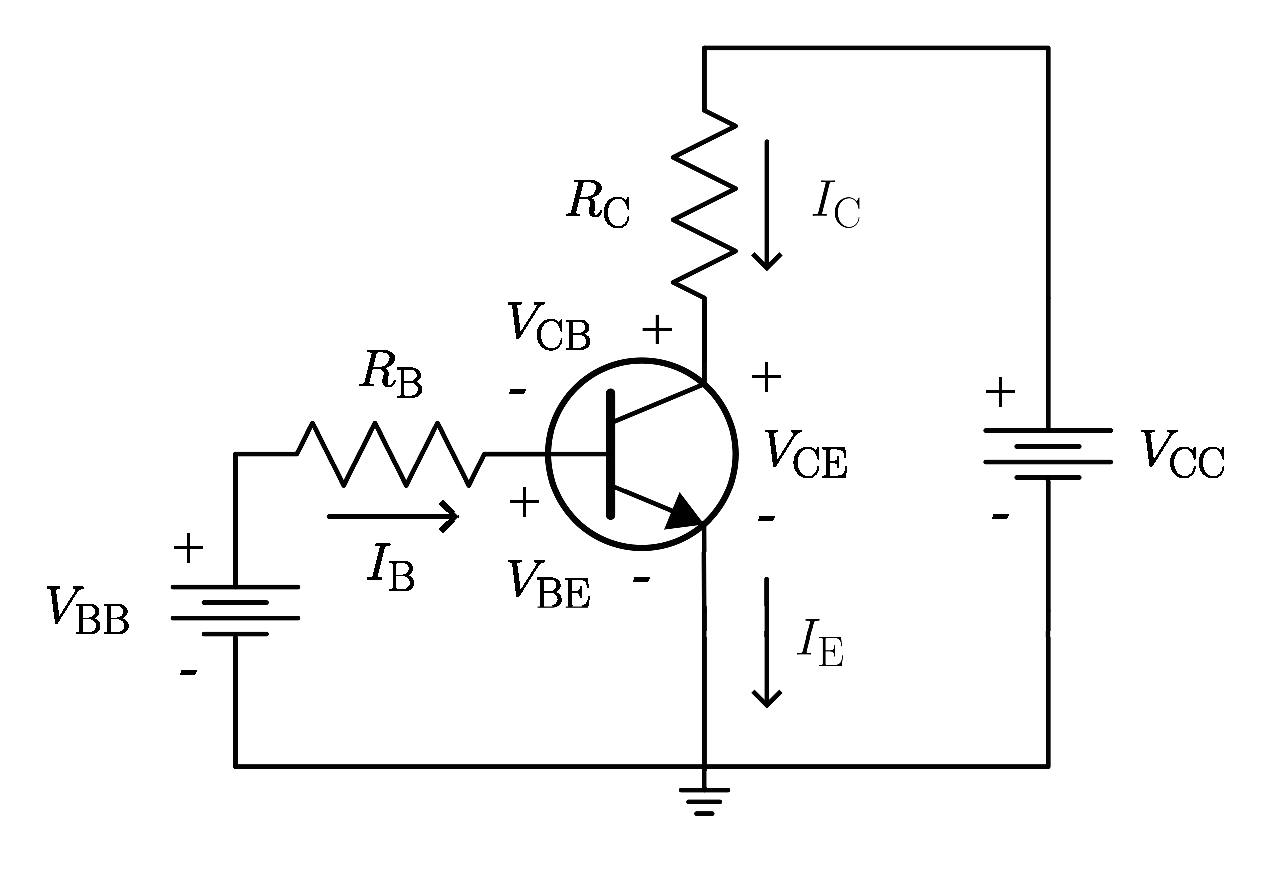
\includegraphics[scale=0.30]{diagramas/figura02.eps}
\caption{Circuito de polarización de cd del transistor \emph{npn}.}
\label{figura02}
\end{figure}

El transistor de unión bipolar presenta ganancia de corriente, lo cual se puede
utilizar para amplificar señales, la \textbf{ganancia} de corriente de cd de un
transistor es el cociente de la corriente de cd del colector ($I_{\text{C}}$)
entre la corriente de cd de la base ($I_{\text{B}}$) y se expresa como
\textbf{beta} de cd ($\beta_{\text{CD}}$).
\begin{equation*}
    \beta_{\text{CD}} = \frac{I_{\text{C}}}{I_{\text{B}}}
\end{equation*}

Existen inconvenientes en el diseño debido a las variaciones de $\beta$ por los
cambios de corriente en el transistor. Además, durante la fabricación del
transistor, se producen variaciones en el valor de beta dentro de un mismo lote
de producción. Por tanto, dos transistores fabricados al mismo tiempo tendrán
diferentes valores de $\beta$, aun en los mismos niveles de corriente
\cite{Savant}.

Cuando la unión base-emisor se polariza en directa, opera como un diodo
polarizado en directa y la caída de voltaje con polarización en directa nominal
es:
\begin{equation*}
    V_{\text{BE}} \cong 0.7 [\text{V}]
\end{equation*}

\subsubsection{Curva característica}
Como el transistor es un dispositivo no lineal, una forma de definir su
operación es usar una serie de curvas características que muestren como varia la
corriente en el colector, $I_{\text{C}}$, con el voltaje en el colector con
respecto al emisor, $V_{\text{CE}}$, con valores especificados de corriente de
base, $I_{\text{B}}$ como puede verse en la \textbf{figura~\ref{figura03}}.

Puede distinguirse la región activa, en esta región el transistor se encuentra
activado. En este modo de trabajo el voltaje que hay entre el emisor y el
colector ($V_{\text{CE}}$) se encuentra entre las regiones de saturación y
corte. La corriente de colector ($I_{\text{C}}$) depende principalmente de la
corriente de base ($I_{\text{B}}$), en esta región el transistor puede funcionar
como amplificador de señales.

\begin{figure}[!ht]
\centering

\includegraphics[scale=0.43]{diagramas/figura03.eps}
\caption{Familia de curvas $V_{\text{CE}}$ contra $I_{\text{C}}$ para varios
valores de $I_{\text{B}}$.}
\label{figura03}
\end{figure}

Un BJT, como cualquier otro dispositivo electrónico, tiene limitaciones en su
operación. Estas limitaciones se establecen en la forma de valores nominales
máximos y normalmente vienen especificadas en la hoja de datos del fabricante.
Típicamente se dan valores nominales máximos de voltaje en el colector con
respecto a la base, voltaje en el colector con respecto al emisor, voltaje en
el emisor con respecto a la base, corriente en el colector y disipación de
potencia.

El producto de $V_{\text{CE}}$ e $I_{\text{C}}$ no debe exceder la disipación de
potencia máxima. Tanto $V_{\text{CE}}$ como $I_{\text{C}}$ no pueden ser máximos
al mismo tiempo. Si $V_{\text{CE}}$ es máximo, $I_{\text{C}}$ se calcula como:
\begin{equation*}
    I_{\text{C}} = \frac{P_{\text{D(máx)}}}{V_{\text{CE}}}
\end{equation*}

\subsubsection{Transistor 2N2222A}
Para la construcción del amplificador se utilizará el transistor BJT tipo
\emph{npn} \textbf{2N2222A}; la hoja de datos de este transistor se detalla en
el \textbf{cuadro~\ref{cuadro01}} \cite{2N2222A}.

\begin{table}[!ht]
\begin{center}
    \begin{tabular}{|c|l|c|c|c|}
    \hline
    \multicolumn{5}{|c|}{\textbf{Valores nominales absolutos máximos}}
    \tabularnewline \hline
    \textbf{Símbolo} &
    \textbf{Parámetro} &
    \multicolumn{2}{|c|}{\textbf{Valor}} &
    \textbf{Unidades}
    \tabularnewline \hline \hline
    $V_{\text{CEO}}$ &
    Voltaje en colector-emisor &
    \multicolumn{2}{|c|}{$40$} & $V$
    \tabularnewline \hline
    $V_{\text{CBO}}$ &
    Voltaje en colector-base &
    \multicolumn{2}{|c|}{$75$} &
    $V$
    \tabularnewline \hline
    $V_{\text{EBO}}$ &
    Voltaje en emisor-base &
    \multicolumn{2}{|c|}{$6.0$} &
    $V$
    \tabularnewline \hline
    $I_{\text{C}}$ &
    Corriente en el colector &
    \multicolumn{2}{|c|}{$600$} &
    $mA$
    \tabularnewline \hline
    $P_{\text{D}}$ &
    Disipación total del dispositivo &
    \multicolumn{2}{|c|}{$625$} &
    $mW$
    \tabularnewline \hline \hline
    \multicolumn{5}{|c|}{\textbf{Características eléctricas (apagado)}}
    \tabularnewline \hline
    \textbf{Símbolo} &
    \textbf{Parámetro} &
    \textbf{Mín.} &
    \textbf{Máx.} &
    \textbf{Unidades}
    \tabularnewline \hline \hline
    $V_{\text{BR(CEO)}}$ &
    Voltaje de ruptura en colector-emisor &
    $40$ &
    $-$ &
    $V$
    \tabularnewline \hline
    $V_{\text{BR(CBO)}}$ &
    Voltaje de ruptura en colector-base &
    $75$ &
    $-$ &
    $V$
    \tabularnewline \hline
    $V_{\text{BR(EBO)}}$ &
    Voltaje de ruptura en emisor-base &
    $6.0$ &
    $-$ &
    $V$
    \tabularnewline \hline
    $I_{\text{CEX}}$ &
    Corriente de corte en el colector &
    $-$ &
    $10$ &
    $nA$
    \tabularnewline \hline
    $I_{\text{CBO}}$ &
    Corriente de corte en la base &
    $-$ &
    $10$ &
    $nA$
    \tabularnewline \hline
    $I_{\text{EBO}}$ &
    Corriente de corte en el emisor &
    $-$ &
    $10$ &
    $nA$
    \tabularnewline \hline \hline
    \multicolumn{5}{|c|}{\textbf{Características eléctricas (encendido)}}
    \tabularnewline \hline
    \textbf{Símbolo} &
    \textbf{Parámetro} &
    \textbf{Mín.} &
    \textbf{Máx.} &
    \textbf{Unidades}
    \tabularnewline \hline \hline
    $h_{\text{FE}}$ &
    Ganancia de corriente en CD & & & $-$
    \tabularnewline
    & $I_C = 0.1mA,\,V_{\text{CE}} = 10V$ &  $35$ &   $-$ & \tabularnewline
    & $I_C = 1.0mA,\,V_{\text{CE}} = 10V$ &  $50$ &   $-$ & \tabularnewline
    & $I_C =  10mA,\,V_{\text{CE}} = 10V$ &  $75$ &   $-$ & \tabularnewline
    & $I_C = 150mA,\,V_{\text{CE}} = 10V$ & $100$ & $300$ & \tabularnewline
    & $I_C = 500mA,\,V_{\text{CE}} = 10V$ &  $40$ &   $-$ &
    \tabularnewline \hline
    $V_{\text{CE(sat)}}$ &
    Voltaje de saturación en colector-emisor & & & $V$
    \tabularnewline
    & $I_C = 150mA,\,I_B = 15mA$ & $-$ & $0.3$ & \tabularnewline
    & $I_C = 500mA,\,I_B = 50mA$ & $-$ & $1.0$ &
    \tabularnewline \hline
    $V_{\text{BE(sat)}}$ &
    Voltaje de saturación en base-emisor & & & $V$
    \tabularnewline
    & $I_C = 150mA,\,I_B = 15mA$ & $-$ & $1.2$ & \tabularnewline
    & $I_C = 500mA,\,I_B = 50mA$ & $-$ & $2.0$ &
    \tabularnewline \hline
    \end{tabular}
\end{center}
\caption{Hoja de datos parcial 2N2222A.}
\label{cuadro01}
\end{table}

\subsubsection{Medición de transistores}
Como se mencionó anteriormente la ganancia de los transistores BJT varían en un
intervalo amplio, por lo cual es recomendable medir individualmente cada uno,
para los cálculos del amplificador.

Se cuenta con un lote de 40 transistores 2N2222A como puede verse en la
\textbf{figura~\ref{figura04}}. Las ganancias ($h_{\text{FE}}$) medidas con un
multímetro en los transistores se detallan en el \textbf{cuadro~\ref{cuadro02}}.

\begin{figure}[!ht]
\centering
\includegraphics[scale=0.12]{diagramas/figura04.eps}
\caption{Lote de transistores 2N2222A.}
\label{figura04}
\end{figure}

\begin{table}[!ht]
\begin{center}
    \begin{tabular}{|c|c|c|c|c|c|c|c|c|c|}
    \hline
    \multicolumn{10}{|c|}{\textbf{$h_{\text{FE}}$}}
    \tabularnewline \hline \hline
    253 & 256 & 297 & 302 & 304 & 264 & 282 & 250 & 279 & 257
    \tabularnewline \hline
    253 & 255 & 289 & 261 & 272 & 282 & 294 & 260 & 264 & 297
    \tabularnewline \hline
    303 & 297 & 280 & 278 & 257 & 255 & 266 & 300 & 295 & 291
    \tabularnewline \hline
    272 & 279 & 262 & 266 & 256 & 285 & 257 & 267 & 289 & 268
    \tabularnewline \hline
    \end{tabular}
\end{center}
\caption{Valor de ganancia medido de cada transistor del lote.}
\label{cuadro02}
\end{table}

La distribución de frecuencias se muestra en la \textbf{figura~\ref{figura05}};
de los cuales se escogieron los tres transistores con mayor valor de ganancia.

\begin{figure}[!ht]
\centering
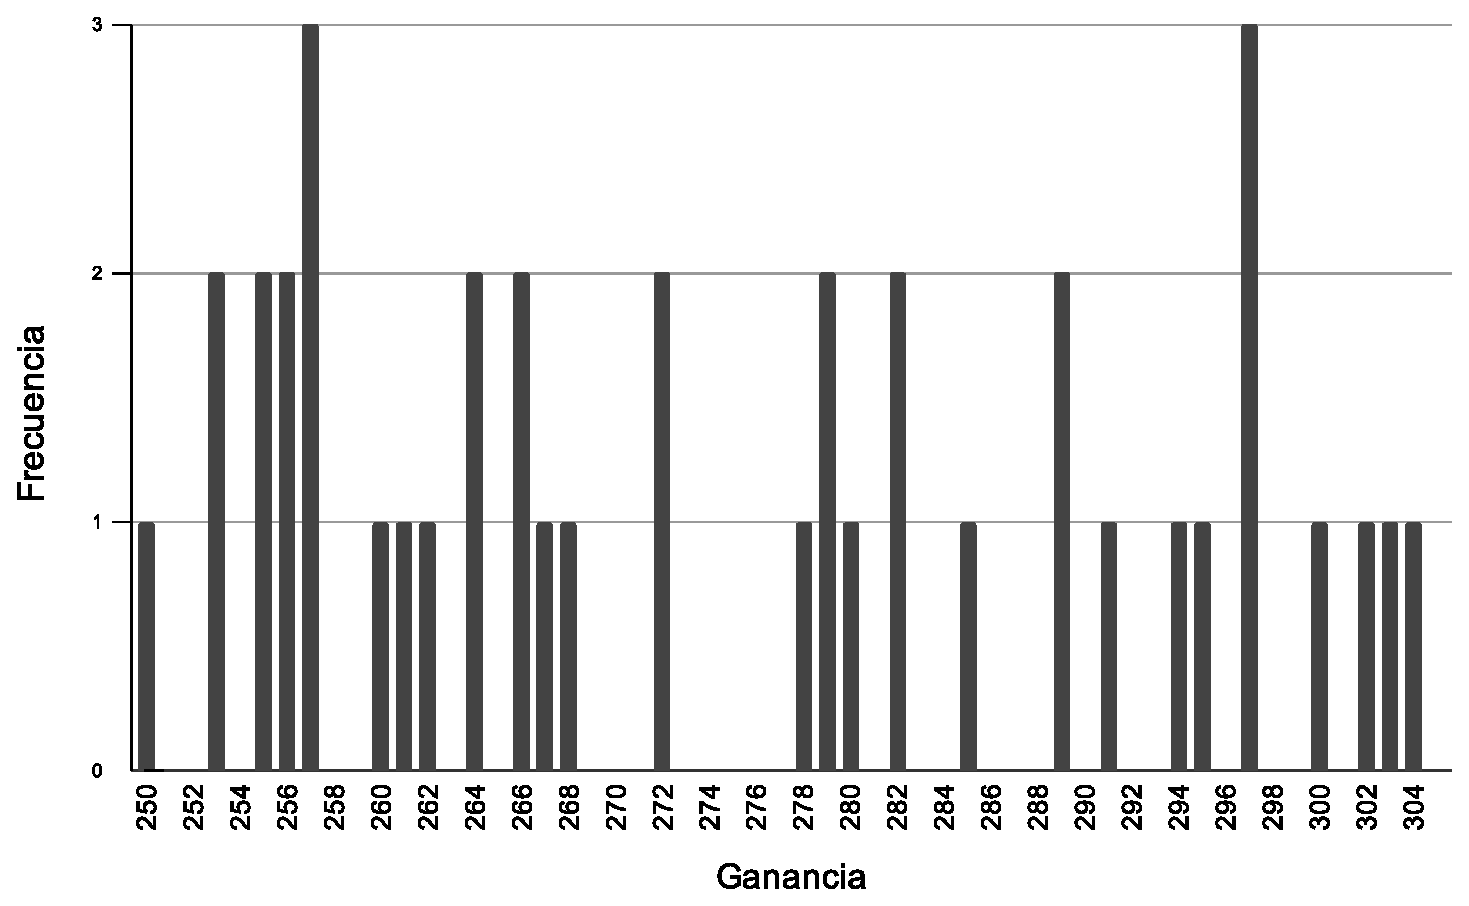
\includegraphics[scale=0.5]{diagramas/figura05.eps}
\caption{Distribución de frecuencia de ganancias de los transistores.}
\label{figura05}
\end{figure}

Por tanto, los transistores a utilizar tienen los parametros descritos en el
\textbf{cuadro~\ref{cuadro03}}.

\begin{table}[!ht]
\begin{center}
    \begin{tabular}{|c||c|c|}
    \hline
    No. & $h_{\text{FE}}$ & $V_{\text{BE}}\,[V]$
    \tabularnewline \hline \hline
    1 & 302 & 0.675
    \tabularnewline \hline
    2 & 303 & 0.676
    \tabularnewline \hline
    3 & 304 & 0.676
    \tabularnewline \hline
    \end{tabular}
\end{center}
\caption{Valores $h_{\text{FE}}$ y $V_{\text{BE}}$ medidos en los transistores.}
\label{cuadro03}
\end{table}

